\documentclass[12pt,letterpaper,final]{article}

\usepackage{Sweave}
\usepackage{graphicx}
\usepackage{natbib}
\usepackage{hyperref}
\usepackage{caption}
\usepackage{rotating}
\usepackage{verbatim}
\usepackage{textcomp}
\usepackage{wasysym}

\setlength{\oddsidemargin}{0in}
\setlength{\textwidth}{6.5in}
%\setlength{\topmargin}{0.5in}
\setlength{\textheight}{22cm}
\setlength{\headheight}{0in}
\setlength{\headsep}{0in}
\setlength{\parskip}{5pt plus 2pt minus 3pt}

\def\thefootnote{\fnsymbol{footnote}}
\setcounter{footnote}{1}

\renewcommand{\baselinestretch}{1.2}
\renewcommand{\labelenumi}{(\roman{enumi})}

\renewcommand{\topfraction}{1.0}
\renewcommand{\bottomfraction}{1.0}
\renewcommand{\textfraction}{0.0}
\renewcommand{\floatpagefraction}{1.0}

\newtheorem{definition}{Definition}
\newtheorem{theorem}{Theorem}
\newtheorem{lemma}[theorem]{Lemma}
\newtheorem{claim}[theorem]{Claim}
\newtheorem{fact}[theorem]{Fact}

% to get nice proofs ...
\newcommand{\qedsymb}{\mbox{ }~\hfill~{\rule{2mm}{2mm}}}
\newenvironment{proof}{\begin{trivlist}
\item[\hspace{\labelsep}{\bf\noindent Proof: }]
}{\qedsymb\end{trivlist}}


\newfont{\msymb}{cmsy10 scaled 1000}

\def\nullset{\mbox{\O}}
\def\R{{I\!\!R}}
\def\C{{I\!\!\!\!C}}
\def\N{{I\!\!N}}

\def\P{\mbox{\msymb P}}


%\parskip 0.1in
\pagenumbering{arabic}    %  Start using 1,2,... as page numbers.
\pagestyle{plain}         %  Page numbers in middle bottom of page.
%\setcounter{page}{80}  % XXXXXXXXXXXXXXXXX
%\setcounter{theorem}{5} % XXXXXXXXXXXXXXXXX
%\setcounter{definition}{10} % XXXXXXXXXXXXXXXXX

\parindent 0in


\begin{document}

\Sconcordance{concordance:hw03_bartschi.tex:hw03_bartschi.Rnw:%
1 161 1 1 2 1 0 5 1 1 5 11 0 1 9 8 0 1 1 4 0 1 2 8 1 1 8 7 0 1 3 2 0 1 %
1 12 0 1 1 4 0 1 2 7 1 1 3 14 0 1 2 1 0 2 1 1 4 3 0 1 3 1 0 1 1 1 3 1 0 %
1 3 1 0 1 4 3 0 1 2 12 0 1 2 9 1 1 3 2 0 1 11 13 0 1 2 14 1 1 2 1 0 1 %
48 51 0 1 2 34 1 1 3 2 0 1 1 1 3 2 0 3 1 5 0 1 1 1 2 1 0 2 1 1 2 1 0 1 %
4 2 0 2 1 1 8 6 0 2 2 1 0 1 1 1 2 1 0 1 5 1 0 1 8 6 0 2 1 1 2 1 4 2 0 3 %
1 1 3 1 0 1 4 1 0 2 3 1 0 1 3 1 0 1 9 12 0 1 4 2 0 1 8 6 0 1 3 1 8 10 0 %
1 2 213 1}


\begin{titlepage}
\vspace*{4.5cm}
\begin{center}
{\LARGE \bf Stat 5810, Section 003} \\[0.5cm]
{\LARGE \bf Statistical Visualization I} \\[0.5cm]
{\LARGE \bf Fall 2018} \\[0.5cm]
{\LARGE \bf Homework 3} \\[0.5cm]
~ \\[2cm]
{\bf ShaunMicheal Bartschi} \\[0.3cm]
{A01975136} \\[0.3cm]
{December 9, 2018} \\[0.3cm]
\end{center}

\thispagestyle{empty}
\vfill
\end{titlepage}

\begin{table}\centering
\begin{tabular*}{6.15in}{@{\extracolsep{\fill}}|llr|} \hline
Stat 5810 Statistical Visualization I & \hspace*{0.5 in} & Fall 2018 \\
 & & \\
\multicolumn{3}{|c|}{
Homework Assignment 3 (11/21/2018)} \\
 & & \\
\multicolumn{3}{|c|}{
40 Points --- Due Sunday 12/9/2018 (via Canvas by 11:59pm)} \\
\hline
\end{tabular*}
\end{table}


\begin{enumerate}

\item (10 Points) Carefully look at the graph below:

\begin{figure}[ht]
\centerline{
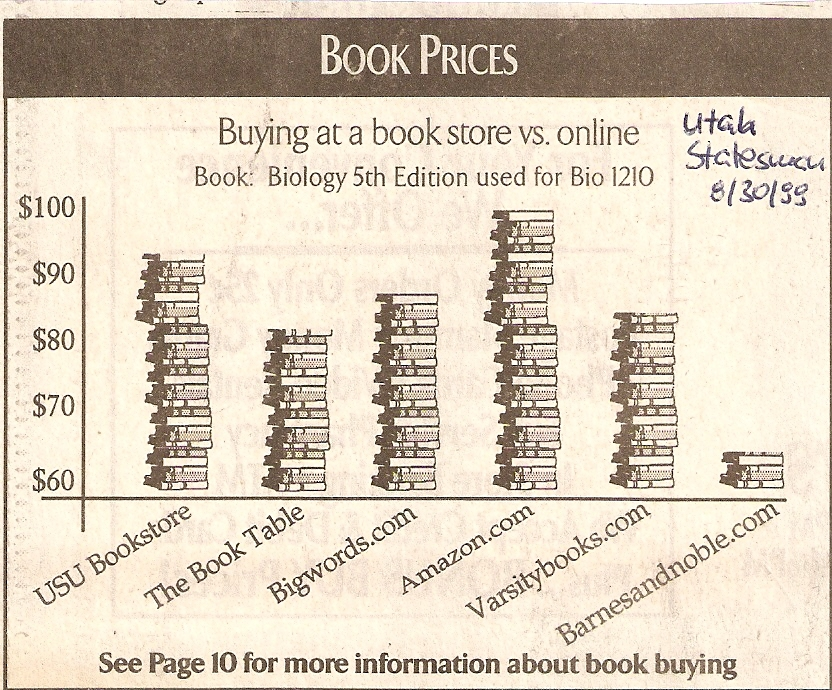
\includegraphics[width=0.5\textwidth]{hw03_q01_Fig1_books.jpg}}
\end{figure}

\begin{enumerate}
\item (3 Points) Explain which rule(s) 
(how to construct a bad graphic) from our lecture notes the graph
designer has followed, i.e., list the rule(s) (number and name)
and explain why it has been followed. Do not blindly list rules (numbers and names)
as you will lose points if you incorrectly quote a rule.
Be sure that you understand the difference between rules 3 and 4.

\item (4 Points) Demonstrate how this poor graph might be improved.
Using the data from the graph (or your best approximation if necessary),
construct a superior representation of the same information, using R,
similar to the improvements from Section~6.2 of our lecture notes.
You can use any R package of your choice to create the improved version.
Include a scan or a photo of the bad graph in your answer,
next to your improved version. Also include your R code.

\item (3 Points) Include a short write--up (about half a page) as to how you 
believe your version improves on the poor original. More specifically,
indicate what you have modified and why this improves the representation
of the underlying data.

\end{enumerate}
\break

\underline{Rules that it breaks:}
\begin{itemize}
  \item Rule 4 (Only Order Matters) - Choosing to represent the bars with offcentered books leads to the impression that the area may be changing in density.
  \item Rule 9 (Alabama First) - It appears that the graph is order from brick and mortar stores (further arranged by distance from campus), and then online book retailers (which appear to be unorganized after this point).
%  \item other - The books obfuscate what data is shown
\end{itemize}

\begin{Schunk}
\begin{Sinput}
> setwd("C:/Users/Shaun/Desktop/StatVis/HW3")
> library(ggplot2)
> library(ggthemes)
> library(grid)
> library(gridExtra)
> library(extracat)
> library(lvplot)
> library(lattice)
> library(scales)
> library(jpeg)
> library(cowplot)
> library(magick)
> book <- data.frame("store" = c("USU Bookstore","The Book Table",
+                                "Bigwords.com","Amazon.com",
+                                "Varsitybooks.com", "Barnesandnoble.com"),
+                    "price" = c(93,80,85,99,82,63))
> book$store <- factor(book$store,levels = book$store[order(book$price)])
> original <- ggdraw() + draw_image("hw03_q01_Fig1_books.jpg",scale=1.5)
> improved <- ggplot(book, aes(x=store,y=price))+geom_col(fill = 'blue', 
+                                                         color = 'black') + 
+   theme(axis.text.x = element_text(angle = 50, hjust = 1), 
+         panel.grid.major.y = element_line(color = 'grey'),
+         panel.grid.minor.y = element_line(color = 'grey')) + 
+   xlab("Purchasing Venue for Biology 5th Edition") + 
+   ylab("Price (As of 1999)") + 
+   ggtitle("Buying at a book store vs. online") + 
+   scale_y_continuous(labels=dollar_format(), breaks = 
+                        c(0,10,20,30,40,50,60,70,80,90,100))
> grid.arrange(original,improved, nrow=1)
\end{Sinput}
\end{Schunk}
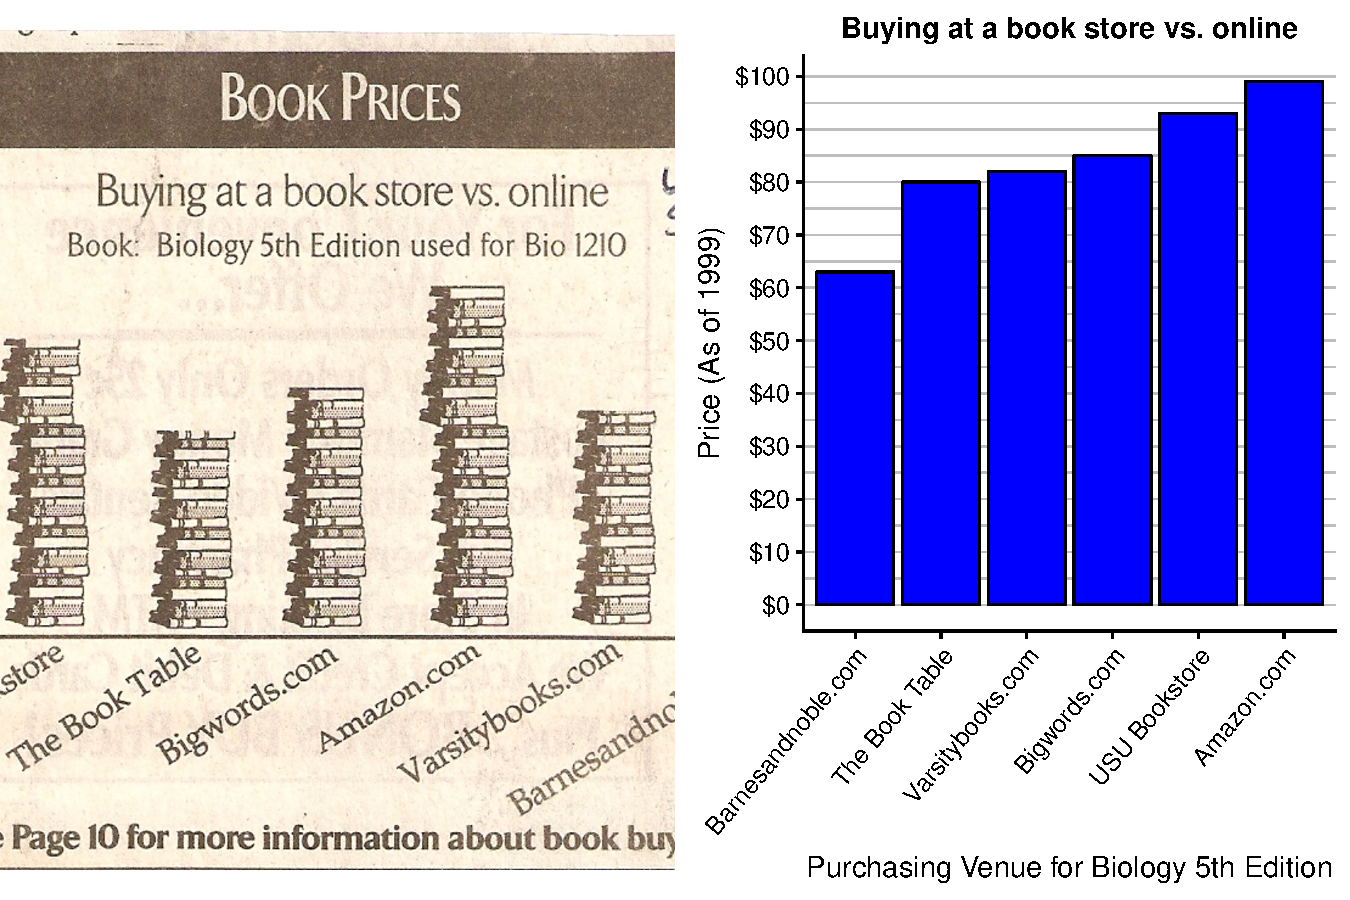
\includegraphics{hw03_bartschi-001}

By rescaling the graph and by placing the sellers in accending order, I believe that I have been able to improve upon th original graph.\\

Now, it is more clear how the various retailers compare in selling prices to one another, the area under the bars is now accurately representative of price, and it is easier to find the relavite price of each of the respective books.
\newpage


\item (10 Points) Carefully look at the graph and text below:

\begin{figure}[ht]
\centerline{
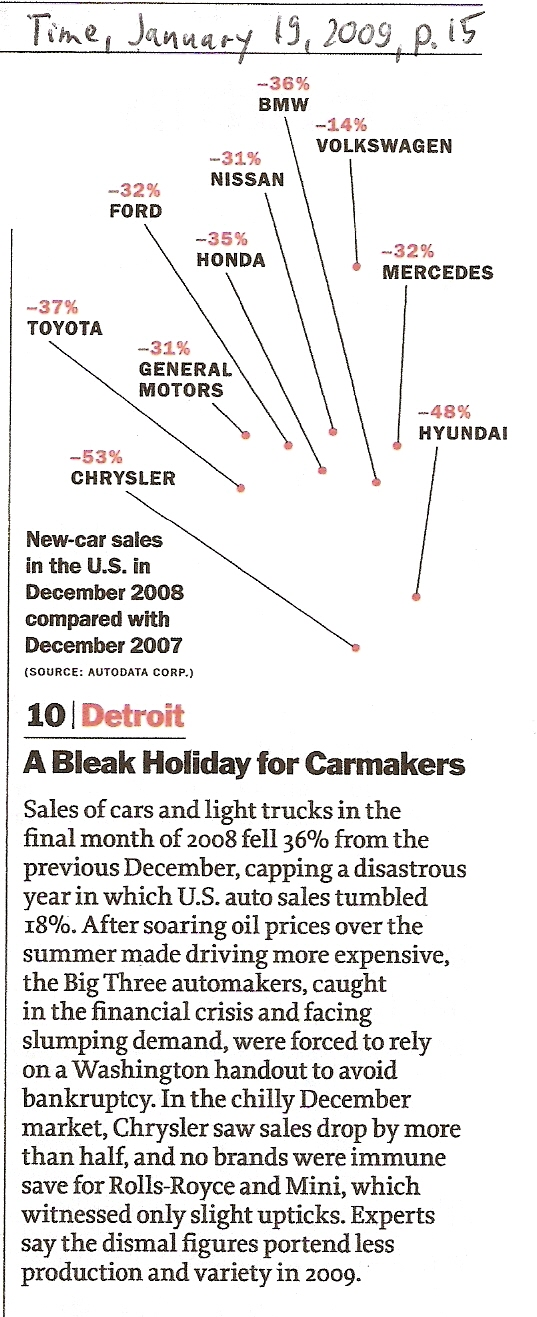
\includegraphics[width=0.45\textwidth]{hw03_q02_Fig2_cars.jpg}}
\end{figure}

Repeat parts (a) through (c) from the previous question for this graph.
When constructing your improved version, keep in mind that these numbers are decreases
(and not increases)!

\break

\underline{Rules that it breaks:}
\begin{itemize}
  \item Rule 5 (Graph Data Out of Context) - 
  \item Rule 9 (Alabama First) - 
  \item Rule 10 (Missing Labels) - 
  \item Rule 12 (Think of a New way to do it) - 
\end{itemize}

\begin{Schunk}
\begin{Sinput}
> original <- ggdraw() + draw_image("p2_clipped.png")
> auto <- data.frame(maker = c("BMW","Volkswagen","Nissan","Ford",
+                              "Honda","Mercedes","Toyota","General Motors",
+                              "Hyundai","Chrysler"),
+                    loss = c(-0.36,-0.14,-0.31,-0.32,-0.35,-0.32,
+                             -0.37,-0.31,-0.48,-0.53))
> auto$maker <- factor(auto$maker,levels = auto$maker[order(-auto$loss)])
> improved <- ggplot(auto, aes(x=maker,y=loss)) + 
+   geom_point(color = 'black',fill = 'red', shape=25) + 
+   theme(axis.text.x = element_text(angle = 50, hjust = 1), 
+         panel.grid.major.y = element_line(color = 'grey'), 
+         panel.grid.minor.y = element_line(color = 'grey')) +
+   scale_y_continuous(labels = percent, breaks = 
+                        c(0,-0.1,-0.2,-0.3,-0.4,-0.5,-0.6), 
+                      limits = c(-0.6,0)) + 
+   xlab("Auto Manufacturer") + 
+   ylab("December Sales Percentage drop in 2008\n(vs previous year)") + 
+   ggtitle("A Bleak Holiday for Carmakers")
> grid.arrange(original,improved, nrow=1)
\end{Sinput}
\end{Schunk}

\includegraphics{hw03_bartschi-002}

By redoing this graph, is has now been done in such a way that graphical interpretation can actually be done on it.  Prior to reploting the data, it was completely unclear what the individual points were meant to represent.  \\

Now, by ordering them in decending order according to losses (as well as using red down facing triangle to represent the loss), the car manufactures losses are now comparable, and the axis are approprately labeled.
\newpage


\item (20 Points) Now you need to find your own bad graph!

\begin{enumerate}
\item (5 Points) Find a bad graph you want to discuss and improve for this homework question.
``Claim'' your bad graph via a personal announcement to me via e-mail or in Canvas. Be specific
which graph you want to improve, in particular if there is more than one bad graph
shown. Include the URL for a graph found on the web, the full reference with page number 
and figure number for a bad graph from a publication, or all necessary details
for a bad graph found in a newspaper, in class materials, etc. 

Web pages, journal articles,
newspapers, magazines, and scholarly books are all appropriate sources.
Good sources for bad graphs are CNN, Time magazine,
the Utah Statesman, Wikipedia, and many other online sites,
but also textbooks and journal papers.

Your bad graph must meet at least one of the rules for bad graphs from Chapter~6
in our lecture notes. I will award extra credit points to all those students
who found graphs with the maximum number of ``approved'' rules for bad graphs
(i.e., if 3 students find bad graphs with 5 rules followed, all 3 students will get
the same extra credit points, but if 1 student finds a bad graph with 6 rules followed,
only that student will get the extra credit points).
Note that listing all 12 rules won't help, as I may only ``approve'' 4 of the
rules for your graph (and you may actually lose points for listing too many unapproved rules).

{\bf Each student must claim a graph by Tuesday 11/27/2018, 11:59pm. Each student must
claim a different graph. If you claim a graph that was previously claimed by someone
else, you must find and claim a different graph.}

Note that numerous web sites with overviews of bad graphs exist.
Some examples are \\
\url{https://www.businessinsider.com/the-27-worst-charts-of-all-time-2013-6}, \\
\url{https://www.biostat.wisc.edu/~kbroman/topten_worstgraphs/}, \\
\url{https://www.buzzfeednews.com/article/katienotopoulos/graphs-that-lied-to-us}, \\
and several more.
{\bf You can't use any graph that is posted on these or any other
bad-graph-collection web sites, books, or other publications.
The goal of this HW is NOT to reuse a bad graph that has already been marked
as bad by someone else, but rather to identify a (new) bad graph when
we see it!}


\item (5 Points) I will collect all proposed bad graphs into a PowerPoint presentation.
Each bad graph is shown on a single page, including the name of the student who claimed it
and the source. {\bf Each student will have a maximum of 2~min to introduce the bad graph
in our last lecture on Thursday 11/29/2018}:
(i) Mention the source of the graph; (ii) indicate the rule(s) that have been followed
to make it a bad graph; and (iii) briefly outline how you are going to improve this graph,
e.g., whether you change the type of the graph, modify the layout, etc.
You should practice in advance that you don't speak longer than 2~min!

{\bf Note: If you are unable to attend class on Thursday 11/29/2018, 
you have two options:
(1) Claim your bad graph by Sunday 11/25/ 2018 and present it in class on
Tuesday 11/27/2018. All other requirements remain the same; or
(2) Call my office number at 435 797 0696 by Tuesday 11/27/2018.
Leave a voice mail, starting with your name, and then
provide the information for (i) to (iii) listed in (b) above. 
I will then play your voice mail in class
on Thursday 11/29/2018 as part of the presentations.

*** In any case, you must contact me in advance via e-mail if you are
not able to attend class on Thursday 11/29/2018. ***}


\item (10 Points) Repeat parts (a) through (c) from the two previous questions for your bad graph.
In your discussion, include the exact source of your bad graph, i.e., the information
you initially sent to me when you claimed your graph.

\end{enumerate}

Bad Graph Coutesy of \url{http://www.gunfacts.info/wp-content/uploads/2013/09/GUNS-IN-OTHER-COUNTRIES-Firearm-Ownership-and-Homicides-Rates-per-Country.png}\\
Data Courtesy of the Guardian\\ \url{https://docs.google.com/spreadsheets/d/1chqUZHuY6cXYrRYkuE0uwXisGaYvr7durZHJhpLGycs/edit}\\

\underline{Original Graph:}\\
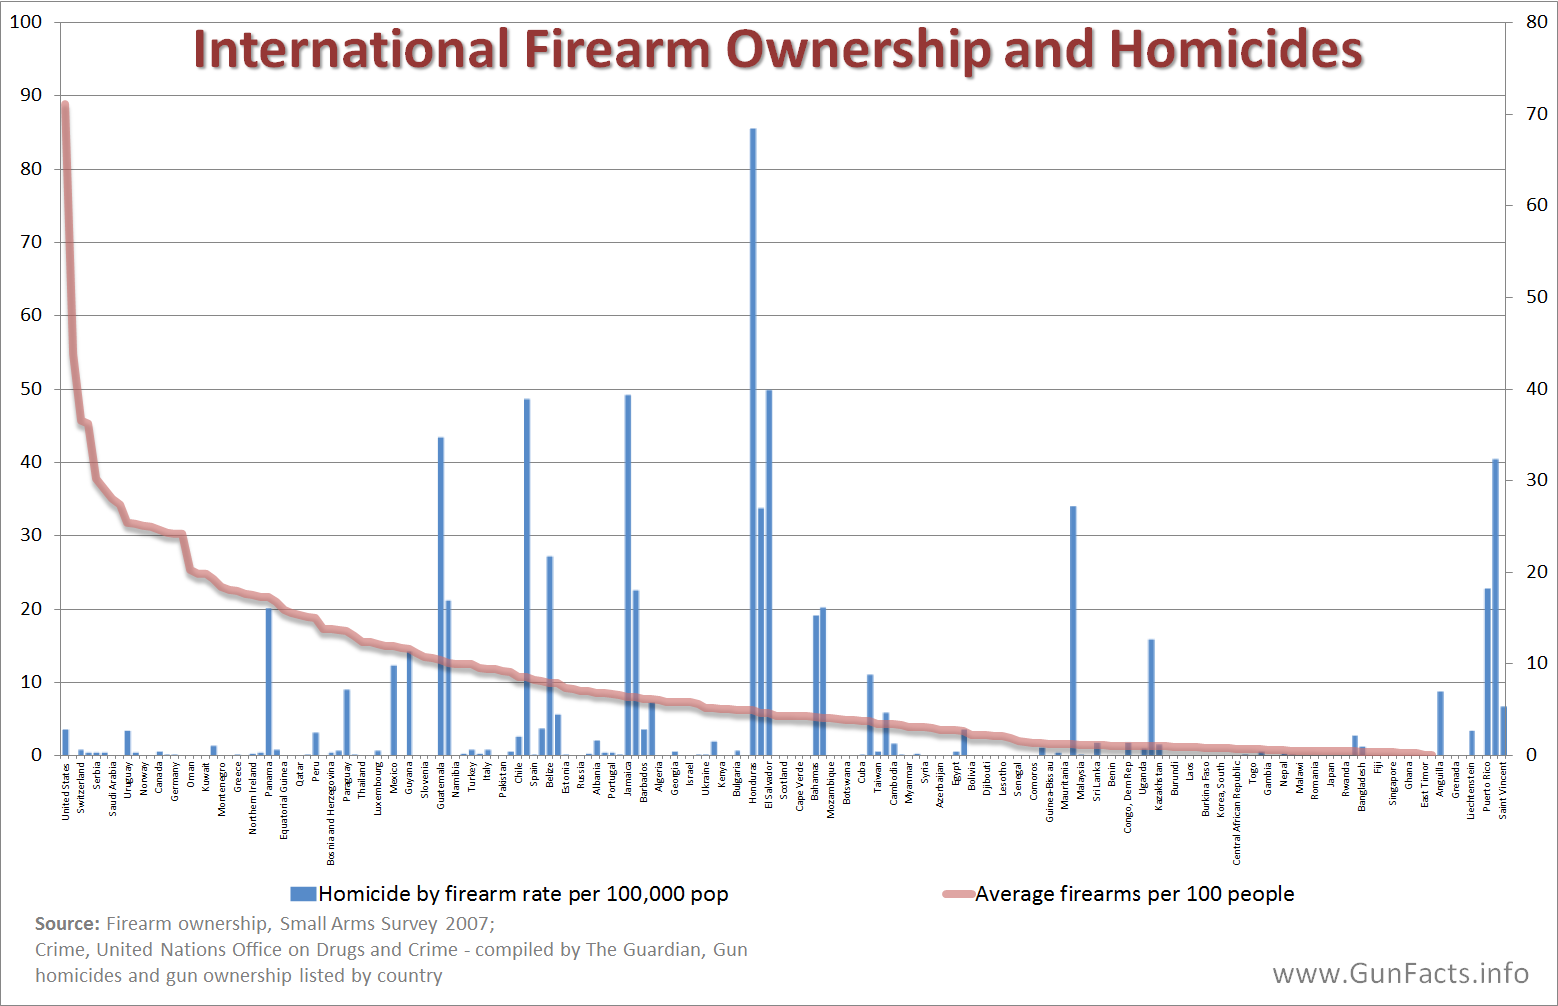
\includegraphics[scale=0.75]{Bad_Graph.png}\\
\underline{Rules that it breaks:}
\begin{itemize}
  \item Rule 7 (Emphasize the trivial) - 
  \item Rule 10 (Label Incompletely) - 
  \item Rule 11 (More is Murkier) - 
\end{itemize}
\underline{Proposed Improved Graph:}\\

\begin{Schunk}
\begin{Sinput}
> dat = read.csv("GunViolence_GunOwnership.csv", header = TRUE, sep=",")
> dat <- dat[!(is.na(dat$Homicide.by.firearm.rate.per.100.000.pop) | 
+                is.na(dat$Average.firearms.per.100.people) | 
+                dat$Average.firearms.per.100.people == "0" | 
+                dat$Homicide.by.firearm.rate.per.100.000.pop == "0"),]
> ownership <- dat$Average.firearms.per.100.people
> homicide <- dat$Homicide.by.firearm.rate.per.100.000.pop
> corr_eqn <- function(x,y, digits = 2) {
+   corr_coef <- round(cor(x, y), digits = digits)
+   paste("italic(r) == ", corr_coef)
+ }
> labels = data.frame(x = 60, y = 12, label = corr_eqn(homicide, ownership))
> loglabels = data.frame(x = 16, y = 1, label = corr_eqn(log(homicide),
+                                                        log(ownership)))
> p1 <- ggplot(dat, aes(x=homicide, y=ownership)) + 
+   geom_point(color = 'red',shape = 1) + 
+   geom_text(data = labels, aes(x = x, y = y,
+                         label = label), parse = TRUE) +
+   xlab("Homicides / 100,000 individuals") +
+   ylab("Average Firearms / 100 individuals") +
+   ggtitle("Original Scale") +
+   theme(plot.title = element_text(hjust = 0.5)) +
+   xlim(0,80) + ylim(0,100)
> p2 <- ggplot(dat, aes(x=homicide, y=ownership)) + 
+   geom_point(color = 'red', shape = 1) +
+   scale_x_continuous(trans='log2',
+     breaks = c(1/64,1/16,1/4,1,4,16,64),
+     labels = trans_format("log2", math_format(2^.x))) + 
+   scale_y_continuous(trans='log2',
+     breaks = c(1/2,1,2,4,8,16,32,64,128),
+     labels = trans_format("log2", math_format(2^.x))) + 
+   annotation_logticks(sides="b") +
+   geom_text(data = loglabels, aes(x = x, y = y,
+                         label = label), parse = TRUE) +
+   xlab("Homicides / 100,000 individuals") +
+   ggtitle("Replotted Logrithmically") +
+   theme(plot.title = element_text(hjust = 0.5),axis.title.y = 
+           element_blank())
> grid.arrange(p1, p2, nrow = 1, 
+              top=textGrob("Demonstrating a Lack of Correlation between\nInternational Gun Ownership & Gun-Related Homicide",
+                           gp=gpar(fontsize=20,font=8)))
\end{Sinput}
\end{Schunk}
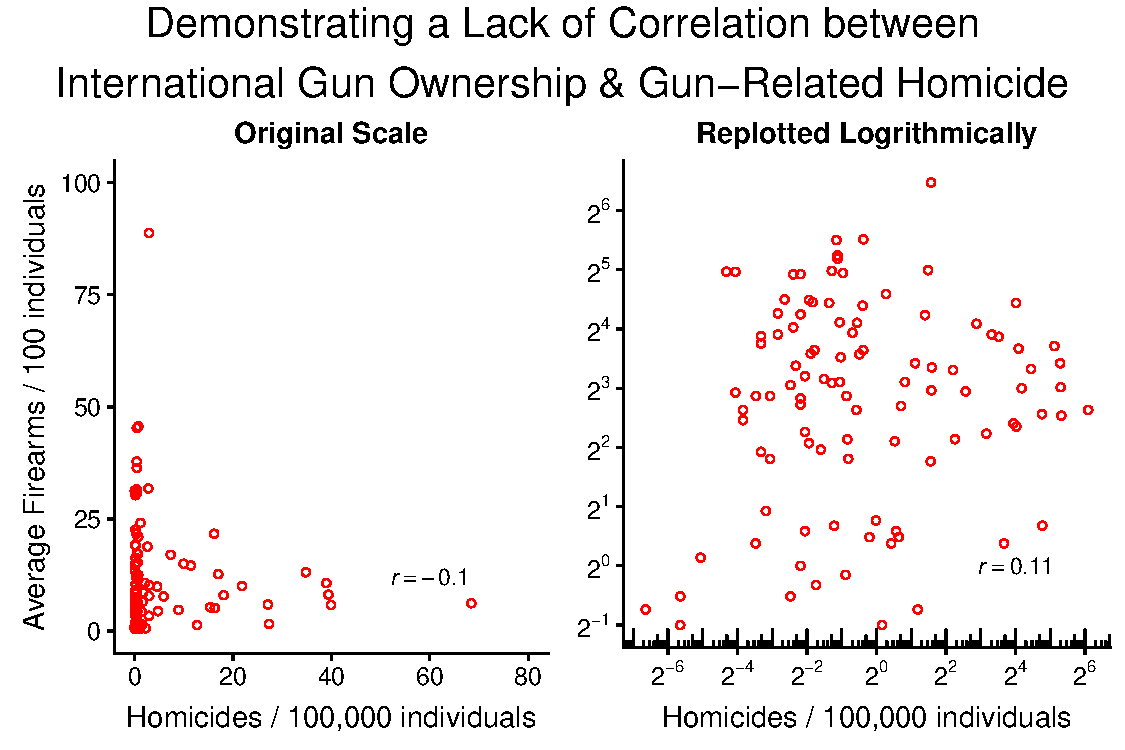
\includegraphics{hw03_bartschi-003}

By showing the data as a scatterplot instead (and excluding the Country the data is describing), we are able to more clearly illustrate that there is no correlation between Gun Homicide and Average Gun ownership.  And by plotting the data on two different scales, we see that even logrithmically, there is no meaningful relationship between the two variables on an international scale.\\ 

Also, this plot is much easier to interprete that meaning.  Including the correlation coefficient for each of them helps to illustrate the statistically insignificant relationship.
\end{enumerate}


\newpage


\noindent{\Large \bf General Instructions}~\\


\begin{enumerate}
\item Create a single html or pdf document, using R Markdown, Sweave, or knitr.
You only have to submit this one document.

\item Include a title page that contains your name, your A-number, the number of
the assignment, the submission date, and any other relevant information.

\item Start your answers to each main question on a new page (continuing with the next
part of a question on the same page is fine). 
Clearly label each question and question part.

\item Before you submit your homework, check that you
follow all recommendations from Google's R Style Guide
(see \url{https://google.github.io/styleguide/Rguide.xml}). 
Moreover, make sure that your R code is consistent, i.e., that you use the same
type of assignments and the same type of quotes throughout your entire homework.

\item Give credit to external sources, such as stackoverflow or help pages. Be specific
and include the full URL where you found the help (or from which help page you got 
the information). Consider R code from such sources as ``legacy code or third-party code'' 
that does not have to be adjusted to Google's R Style (even though it would be nice,
in particular if you only used a brief code segment).

\item {\bf Not following the general instructions outlined above will result in point deductions!}

\item For general questions related to this homework, please
use the corresponding discussion board in Canvas! I will try to
reply as quickly as possible. Moreover, if one of you knows
an answer, please post it. It is fine to refer to web pages
and R commands, but do not provide the exact R command with all required arguments
or which of the suggestions from a stackoverflow web page eventually worked for you! 
This will be the task for each individual student!

\item Submit your single html or pdf file via Canvas by the submission deadline.
Late submissions will result in point deductions as outlined on the syllabus.

\end{enumerate}


\end{document}

